\documentclass[aspectratio=43]{beamer}
\usetheme{Copenhagen}
\setbeamertemplate{navigation symbols}{} % remove pdf navigation controls
\RequireXeTeX

\usepackage{hyperref}
\usepackage{fontspec}
\usepackage{graphicx}
\usepackage{beamergitcolors}
\usepackage{beamergitfonts}
\usepackage{multicol}
\usepackage{nicelistings}

\title{Git and Version Control}
\subtitle[GatorLUG]{GatorLUG: Gainesville Linux Users Group}
\author{Benjamin Woodruff}
\institute{University of Florida}
\date{September 19\textsuperscript{th}, 2012}
\titlegraphic{
\includegraphics[height=2cm]{resources/git_icon_ice.pdf}}

\begin{document}

\frame{\maketitle}

\begin{frame}{Disclaimers}
    \begin{itemize}
    \item A large part of this talk is based on my own personal views and
        opinions, which you may not agree with
    \item Some information may be incorrect. Feel free to correct me. Send me a
        pull-request on github after the talk!
    \item This talk makes massive sweeping generalizations about lots of things
    \item This talk is focused on git. Discussion about other VCS systems is
        only for comparison, and to give us something else interesting to talk
        about
    \end{itemize}
\end{frame}

\section{Version Control Overview}

\begin{frame}{What is a Version Control System (VCS)?}
    Retains the history of a project (so that you don't have to!)
    \begin{itemize}
    \item Turn this:
        \begin{scriptsize}
        \begin{multicols}{3}
        \texttt{my\_project} \\
        \texttt{my\_project\_5e} \\
        \texttt{my\_project\_dontuse} \\
        \texttt{my\_project\_extras} \\
        \texttt{my\_project\_for\_prof} \\
        \texttt{my\_project\_old} \\
        \texttt{my\_project\_refactor} \\
        \texttt{my\_project\_speedup}
        \end{multicols}
        \end{scriptsize}
        \ldots into one unified structured directory!
    \item Forgot what it was you removed 6 months ago? Look it up!
    \item Something causing a regression? \texttt{git-bisect}!
    \end{itemize}
    \begin{flushright}
        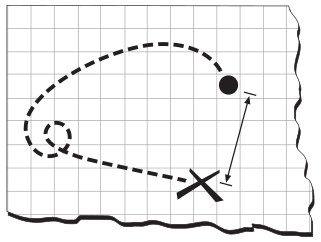
\includegraphics[height=2cm]{resources/mapping_history.pdf}
    \end{flushright}
\end{frame}

\begin{frame}{What is a Version Control System (VCS)?}
    Allows others to collaborate with you over the internet
    \begin{itemize}
    \item Sites like Github, Google Code, and Gitorious are great for this
    \item You can do things in private too
        \begin{itemize}
        \item Github (along with many others) offers paid private hosting
        \item You can use git remotely on any server with ssh
            \begin{itemize}
            \item You can use Gitolite and Gitweb to make your own personal
                Github!
            \end{itemize}
        \end{itemize}
    \item Are you a hermit and don't have a server or money? You can do things
        locally too!
    \end{itemize}
    \begin{flushright}
        \includegraphics[height=2cm]{resources/time_clock.pdf}
    \end{flushright}
\end{frame}

\begin{frame}{Who Uses Version Control?}
    \begin{itemize}
    \item Nearly every major software company
    \item Independent software developers
    \item Systems Administrators
    \item Graphics Designers
    \end{itemize}
    Version control has many obvious uses, and many more less-than-obvious uses
    (such as \texttt{git-annex}, a file-management tool).
    \begin{center}
        \includegraphics[height=3cm]{resources/git_annex.pdf}
    \end{center}
\end{frame}

\subsection{Centralized Version Control}

\begin{frame}{Centralized Version Control Systems}
    Examples: Subversion, CVS
    \begin{itemize}
    \item More traditional, simpler to think-about model
    \item Tend to work better with large binary files
    \item Sometimes uses locking to solve issues with multiple contributors
    \item Merging can often be complicated
        \begin{itemize}
        \item Apparently newer versions of Subversion are better at merging, but
            still have a lot of flaws
        \end{itemize}
    \end{itemize}
    \begin{center}
        \includegraphics[width=.7\linewidth]{resources/subversion_logo.pdf}
    \end{center}
\end{frame}

\begin{frame}{How Centralized Version Control Works}
    \begin{itemize}
    \item A linear history is stored by the VCS, and revisions are typically
        referred to by a sequential number
    \item Requires a centralized server to store the whole history
        \begin{itemize}
            \item This could be run locally
            \item Most history-related operations will require network access
            \item Since we don't copy everything initially, the initial checkout
                is faster
        \end{itemize}
    \end{itemize}
    \begin{center}
        \includegraphics[width=.7\linewidth]%
                        {resources/centralized_vs_decentralized.pdf}
    \end{center}
\end{frame}

\subsection{Distributed Version Control}

\begin{frame}{Distributed Version Control Systems}
    Examples: git, Mercurial, Bazaar, GNU Arch
    \begin{itemize}
    \item Represents a non-linear progression of the code
    \begin{itemize}
        \item Git uses hashes and tags to refer to commits
        \item State of the code is defined only by a sequence of differences
    \end{itemize}
    \item Everyone owns the entire repository
    \begin{itemize}
        \item Slower initial clone, but faster operations on repository history
        \item Storing large binary files is awkward as a result, since everyone
            has to download every copy that ever existed of the binary
            \footnote{unless the VCS implements binary diffing, which most
                      don't}
    \end{itemize}
    \item Distribution via pushing and pulling from other repositories
        \begin{itemize}
        \item No explicit hierarchy
        \end{itemize}
    \item No lock-in. Switching hosting providers takes minutes
    \item Forking is trivial
    \end{itemize}
\end{frame}

\begin{frame}{Why a Non-Linear Progression?}
    \begin{quotation}
        People assume that time is a strict progression of cause to effect. But
        actually from a non-linear, non-subjective viewpoint it's more like a
        big ball of wibbly-wobbly timey-wimey\ldots stuff.

        --- The 10th Doctor (Doctor Who)
    \end{quotation}
    \begin{flushright}
        \includegraphics[height=2cm]{resources/ball_of_yarn.pdf}
    \end{flushright}
\end{frame}

\begin{frame}{Why a Non-Linear Progression?}
    \begin{itemize}
    \item Software isn't developed linearly. It's not a path from A-to-B.
        Software is organic and living
    \item Feature branches, unstable and nightly versions, and experimental
        changes should all be tracked
    \item Different people work on projects, and they work at different paces
    \item We want cheap branching and merging!
        \begin{itemize}
        \item Since code is just a long sequence of changes, you only need to
            which changes you want, not the actual code to make a branch.
            Changes (or commits) can be shared between branches, and are managed
            somewhat independently
        \end{itemize}
    \item But I like my linear software development style!
        \begin{itemize}
        \item DVCS doesn't force you, it just gives you the option
        \end{itemize}
    \end{itemize}
\end{frame}

\section{Introduction to Git}

\begin{frame}{Git Influences and Motivations}
    \begin{itemize}
    \item Inspired by BitKeeper and Monotone
        \begin{itemize}
        \item Distributed
        \item Optimized for common workflows
        \end{itemize}
    \item Designed to handle the scale requirements of managing the Linux kernel
        \begin{itemize}
        \item Fast, minimalistic, and transparent
        \item Strong (and cryptographically secure) safeguards against
            corruption and tampering
        \end{itemize}
    \item Named after Torvalds, who considers himself a ``git''
        \begin{itemize}
        \item "the stupid content tracker"
        \end{itemize}
    \end{itemize}
    \begin{flushright}
        \includegraphics[height=2cm]{resources/tux.pdf}
    \end{flushright}
\end{frame}

\begin{frame}{Following Along}
    The example repository we'll make is available on github. You can clone it
    locally with: \\
    \begin{small}
    \texttt{git clone https://github.com/GatorLUG/git-talk-example.git}
    \end{small}

    You can find the github page at:
    \url{https://github.com/GatorLUG/git-talk-example}
    
    \begin{center}
        \includegraphics[height=3cm]{resources/put_on_3d_glasses.jpg}
    \end{center}
\end{frame}

\subsection{\texttt{git init}}

\begin{frame}{git init}
    Magically turns a preexisting directory into a git repository
    \begin{itemize}
    \item git's internal tracking information is stored in a new
        ``\texttt{.git}'' directory within the repository:
        \begin{footnotesize}
        \begin{multicols}{4}
            \texttt{branches/} \\
            \texttt{config} \\
            \texttt{description} \\
            \texttt{HEAD} \\
            \texttt{hooks/} \\
            \texttt{info/} \\
            \texttt{objects/} \\
            \texttt{refs/}
        \end{multicols}
        \end{footnotesize}
    \item Git performs agressive deduplication and diffing to reduce size
    \end{itemize}
    The new repository has no state. Let's put something in it!
\end{frame}

\subsection{\texttt{git add} and \texttt{git rm}}

\begin{frame}{A Normal Directory}
    \begin{itemize}
    \item Anything outside of \texttt{.git/} is called your "working directory"
    \item Until you have something new to commit, you can treat it like a normal
        folder.
    \end{itemize}
    Let's put some files in our working directory
    \begin{center}
        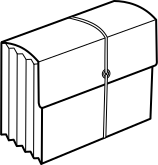
\includegraphics[height=2cm]{resources/dossier.pdf}\hspace{.5cm}%
        
\includegraphics[height=2cm]{resources/dossier_folder.pdf}
    \end{center}
\end{frame}

\begin{frame}[fragile]{bashrc}
    \lstinputlisting[language=bash]{example_files/bashrc_initial}
\end{frame}

\begin{frame}[fragile]{installer.sh}
    \lstinputlisting[language=sh]{example_files/installer.sh}

    We can go ahead and give this file executable permissions:\\
    \texttt{chmod +x installer.sh}

    \begin{flushright}
        \includegraphics[height=3cm]{resources/installer.png}
    \end{flushright}
\end{frame}

\begin{frame}[fragile]{git status}
    We can use \texttt{git status} to check our current state:

    \lstinputlisting[numbers=none, basicstyle=\ttfamily\tiny]
                    {example_files/status_initial_working_directory}

    Our working directory is currently ``dirty''. Let's make git track these
    files\ldots
    
    \begin{flushright}
        \includegraphics[height=2cm]{resources/stethoscope.pdf}
    \end{flushright}
\end{frame}

\begin{frame}{git add - Add file contents to the index}
    \begin{itemize}
    \item Git has a unique feature: The staging area
        \begin{itemize}
        \item Exists between the working directory and the datastore
        \item Allows us to view what's going to be committed before we commit
        \item If we prefer, we can chose to commit only a portion of the working
            directory
        \end{itemize}
    \item We can use \texttt{git add} to add items to the staging area
    \end{itemize}

    Let's add both the files we made to the staging area. We can use:
    \begin{itemize}
    \item \texttt{git add .}
        \begin{itemize}
        \item Adds the current directory (or rather, it's contents recursively)
              the staging area
        \end{itemize}
    \item or \texttt{git add bashrc installer.sh}
        \begin{itemize}
        \item Adds the files explicitly and independently
        \end{itemize}
    \end{itemize}
\end{frame}

\begin{frame}{git rm - Remove from the working tree and index}
    \textbf{Example Usage:} \texttt{git rm src/ugly\_solution.c}
    \begin{itemize}
    \item Stages the removal of a file, and removes it from the working tree
        \begin{itemize}
        \item \texttt{git rm --cached my\_file.py} will only stage the removal,
            not deleting the file
        \end{itemize}
    \item Use this instead of \texttt{rm} or after \texttt{rm}
    \item \texttt{git add .} won't remove files, but \texttt{git add -u .}
        \textit{will} do so automatically
    \end{itemize}
    \begin{flushright}
        \includegraphics[height=2cm]{resources/white_trash.png}
    \end{flushright}
\end{frame}

\subsection{\texttt{git commit}}

\begin{frame}{git commit - Record changes to the repository}
    Committing is easy as running \texttt{git commit} (no extra arguments
    needed!)

    This will spawn a your text editor (defined by the
    \texttt{\textdollar{}EDITOR} environment variable) for you to write your
    commit message. By convention:

    \begin{itemize}
    \item The first line should be 50 characters or less, and should
        provide a short summary
    \item There should be a short but detailed explaination in the next
        paragraph (separated by an empty line). You should wrap to 72
        characters
    \item You can write more paragraphs if you want. Just remember that
        the most important details should be listed first. Commits
        messages should be easily skimmed. You may wish to use bullets.
    \end{itemize}
\end{frame}

\begin{frame}{Example Commit Message}
    \lstinputlisting[numbers=none, basicstyle=\ttfamily\tiny]%
        {example_files/commit_message}
    
    \begin{footnotesize}
    Source: \\
    \url{http://tbaggery.com/2008/04/19/a-note-about-git-commit-messages}
    \end{footnotesize}
\end{frame}

\begin{frame}{A Commit Message for our Previous Example}
    We first run \texttt{git commit}, and then enter

    \lstinputlisting[numbers=none, basicstyle=\ttfamily\tiny]%
        {example_files/initial_commit_message}
    
    We can save and close this file to actually perform the commit.
    
    \vspace{.5cm}

    \begin{footnotesize}
    \textbf{Protip:} For short commit messages, you can use\\
    \texttt{git commit -m "My Commit Message"}\\
    This is not recommended however, as the commit will have no body.
    \end{footnotesize}

    \vspace{.5cm}
    
    \begin{footnotesize}
    \textbf{Protip:} If you make a typo or forget a file, you can always amend
    your last commit with \texttt{git commit --amend} before you push it.
    \end{footnotesize}
\end{frame}

\section{Becoming Productive with Git}

\subsection{\texttt{git branch} and \texttt{git checkout}}

\begin{frame}{Why do I care about Branches?}
    \begin{itemize}
    \item Branches are good for:
        \begin{itemize}
        \item Experimental features
        \item Unstable/Stable versions
        \item Somewhere to play with git
        \end{itemize}
    \item Branching in git is intentionally cheap: \textit{\textbf{do it!}}
    \item Branches are treated equally
    \end{itemize}
    
    \begin{center}
        \includegraphics[height=3cm]{resources/branching_illustration.png}
    \end{center}
\end{frame}

\begin{frame}{No Limit to Structure}
    \begin{center}
        \includegraphics[width=.9\linewidth]{resources/branching_complex.png}
    \end{center}
\end{frame}

\begin{frame}{git branch - List, create, or delete branches}
    \begin{itemize}
    \item Running \texttt{git branch} with no arguments will list the current
        branches
        \begin{itemize}
        \item The default branch (which can be deleted) is called ``master''
        \item An asterisk is used to mark the current branch
        \end{itemize}
    \item You can specify a branch name, and git will create it, basing it on
        the currently checked out branch
        \begin{itemize}
        \item \texttt{git branch new-stuff}
        \item If you'd like the new branch to be based on a branch not currently
            checked out: \texttt{git branch old-stuff new-stuff}
        \end{itemize}
    \end{itemize}

    \begin{flushright}
        \includegraphics[height=2cm]{resources/git_icon.pdf}
    \end{flushright}
\end{frame}

\begin{frame}{git checkout - Checkout a branch or paths to the working tree}
    So we made a new branch, now let's set the working directory to that branch
    \begin{itemize}
    \item \texttt{git checkout new-branch}
    \item You can check that the branch was changed with \texttt{git branch}
    \item You can branch and checkout in one step
        \begin{itemize}
        \item \texttt{git checkout -b new-stuff}
        \end{itemize}
    \item \texttt{git checkout} isn't just for branches, it can also be used to
        check out commits or tags. Think of it as a time-machine
    \item You can use \texttt{git checkout} to check out only a specific file or
        directory at a time
    \end{itemize}
\end{frame}

\begin{frame}[fragile]{Populating our Example with a History}
    To give us something to play around with, let's give our example repository
    a history\ldots

    \vspace{.5cm}

    \texttt{\textbf{bash\_aliases}}
    \lstinputlisting[basicstyle=\ttfamily\tiny, language=bash]%
        {example_files/bash_aliases}
    
    \texttt{\textbf{installer.sh}}
    \lstinputlisting[basicstyle=\ttfamily\tiny, language=sh]%
        {example_files/installer_aliases.sh}

    We'll branch, checkout, add this, and then commit.
\end{frame}

\subsection{\texttt{git log}}

\begin{frame}{git log - Show commit logs}
    There's no point in having a history if you can't keep track of it!
    
    Running \texttt{git log} over our new branch gives us:
    \lstinputlisting[numbers=none, basicstyle=\ttfamily\tiny]%
        {example_files/log_aliases}
\end{frame}

\begin{frame}{Jumping back in time}
    Let's run \texttt{git checkout d3ca0f}\footnote{You only need to write
    enough characters of the hash for git to be able to identify this commit}

    \lstinputlisting[numbers=none, basicstyle=\ttfamily\tiny]%
        {example_files/detached_head}

    When we're done, we can jump back to the future with:\\
    \texttt{git checkout aliases}\\
    (where aliases is the name of the current branch)
\end{frame}

\begin{frame}[fragile]{What is the HEAD?}
    \begin{itemize}
    \item A special reference that points to the currently checked out
        branch and commit
        \begin{itemize}
        \item Can be used (almost) anywhere a commit hash is expected
        \end{itemize}
    \item \texttt{HEAD\textasciitilde{}1}, \texttt{HEAD\textasciitilde{}2}, etc
        points to the currently checked out commit, minus one, or two commits
        \begin{itemize}
        \item Useful for quickly referencing that last commit you made
        \end{itemize}
    \item You can see where HEAD has been with \texttt{git reflog HEAD}
        \begin{itemize}
        \item You can reference previous states of the \texttt{HEAD} if you
            want, as listed by \texttt{git reflog} with \verb|HEAD@{1}|,
            \verb|HEAD@{2}|, etc
        \end{itemize}
    \end{itemize}
    \begin{flushright}
        
\includegraphics[height=2cm]{resources/deer_head.pdf}
    \end{flushright}
\end{frame}

\subsection{\texttt{git merge} and \texttt{git cherry-pick}}

\begin{frame}{git merge - Join development histories together}
    \begin{itemize}
    \item Brings the current branch up to date with another history in another
        branch
    \item Can be used to either merge an entire branch, or just another branch
        up to a certain commit
    \end{itemize}
    \textbf{Example:} \texttt{git merge other-stuff}
    \begin{itemize}
    \item Normally, git will attempt to automatically merge the commit for you.
        Certain complex situations will cause it to fail. When this happens
        \begin{itemize}
        \item Git will tell you what files it failed to merge
        \item Open the file(s), and find where git has marked a merge conflict
        \item Rewrite the code how you want it
        \item \texttt{git status} will let you know when you are ready to commit
        \item Run \texttt{git commit} to write back the ``merge commit''
        \end{itemize}
    \end{itemize}
\end{frame}

\begin{frame}{git cherry-pick - Apply the changes introduced by some existing
              commits}
    Like \texttt{git merge}, but for only specific commits (instead of a whole
    branch, or an entire history of commits)

    \begin{itemize}
    \item Commits can be picked out of order
    \item Merge conflicts are handled identically to \texttt{git merge}
    \end{itemize}

    \textbf{Example Usage:} \texttt{git cherry-pick 08a1fa}
    \begin{flushright}
        \includegraphics[height=3cm]{resources/cherries.pdf}
    \end{flushright}
\end{frame}

\section{Collaborating with Git}

\subsection{Github}

\begin{frame}{Github}
    \begin{itemize}
    \item Most popular git hosting site in the world
        \begin{itemize}
        \item Other hosting sites exist, and are worth checking out
        \end{itemize}
    \item Easy to use
    \item Provides large amounts of documentation
    \item Signing up for an account is easy
        \begin{itemize}
        \item They'll guide you through setting up an ssh key
        \end{itemize}
    \end{itemize}
    \begin{center}
        \includegraphics[height=2cm]{resources/github_logo.pdf}
    \end{center}
\end{frame}

\subsection{Configuring Git}

\begin{frame}{\textasciitilde/.gitconfig}
    \begin{itemize}
    \item Refered to as your "global" config
        \begin{itemize}
        \item If you wish, you can set options on a per-repository basis
        \end{itemize}
    \item Can also be edited indirectly with \texttt{git config --global}
    \item Edit with \texttt{git config --global -e}, or just open it up with
        your favorite text editor
        \begin{itemize}
        \item When I say ``your favorite text editor'', I mean \texttt{vim}
            \begin{itemize}
            \item Only idiots (with Lord Stallman being an exception) use emacs
            \end{itemize}
        \end{itemize}
    \end{itemize}
    \begin{center}
        \includegraphics[height=1cm]{resources/vim_logo.pdf}
        \includegraphics[height=2cm]{resources/vim_logo.pdf}
        \includegraphics[height=3cm]{resources/vim_logo.pdf}
        \includegraphics[height=2cm]{resources/vim_logo.pdf}
        \includegraphics[height=1cm]{resources/vim_logo.pdf}
    \end{center}
\end{frame}

\begin{frame}{VIM VIM VIM VIM VIM VIM}
    \begin{center}
        \includegraphics[height=7cm]{resources/vim_logo.pdf}
    \end{center}
\end{frame}

\begin{frame}{Example \textasciitilde/.gitconfig}
    \lstinputlisting{example_files/gitconfig}
\end{frame}

\begin{frame}{Pushing a Repository to Github}
    Demo\ldots
\end{frame}

\section{}
\begin{frame}{Questions?}
\begin{center}
    \includegraphics[height=3cm]{resources/gatorlug_logo.png}
\end{center}
\end{frame}

\end{document}
